%%%Slides
    \begin{figure} \centering  % [h!]  [!ht]
        \caption{ ~Simulated dynamics from a SIR model of stock investors}
        \label{fig:sir_simulate}
        \centerline{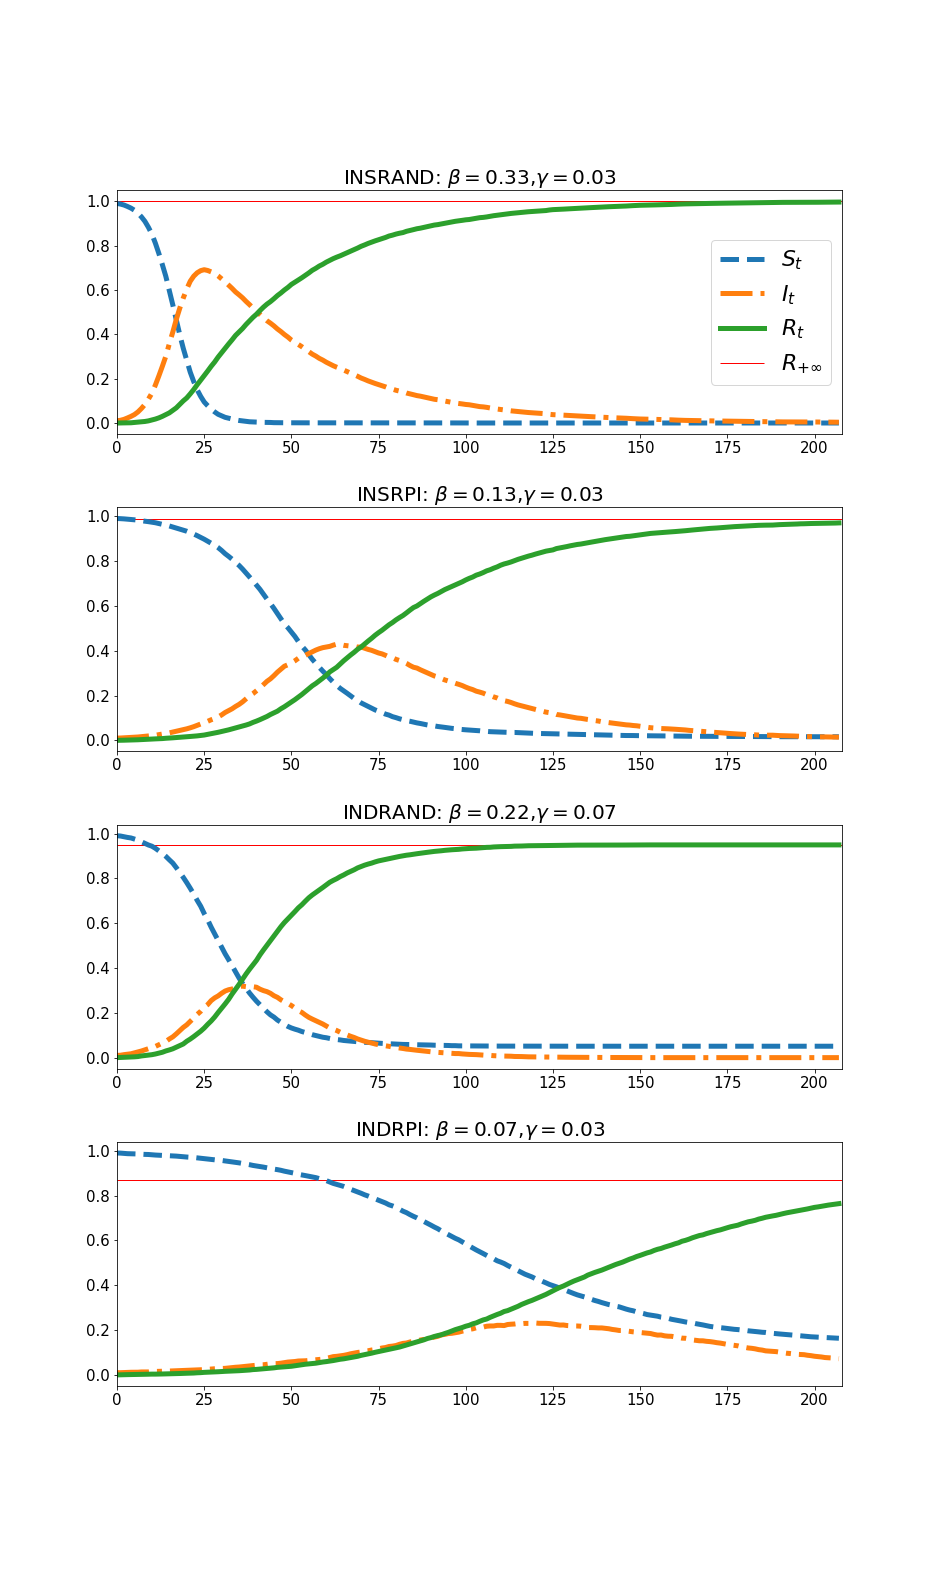
\includegraphics[width=0.85\textwidth,height=0.85\textheight]{./figures/sir_simulate}}
        \begin{flushleft}
            {\footnotesize The four figures respectively simulate an SIR model under calibrations corresponding to \cite{shiller1989survey}'s parameter estimates for (1) institutional investors for a randomly selected stock (INSRAND); (2) institutional investors for a rapidly rising stock (INSRPI); (3) individual investors for a random stock (INDRAND); and (4) individual investors for a rapidly rising stock (INDRPI). The susceptible population {\Susceptible} is dashed; dash-dot shows the size of the {\Infected} compartment, and the recovered population {\Recovered} is solid.  The horizontal thin solid line corresponds to the limiting size of compartment of $R$ in the long run.  To reproduce these figures, see the companion \href{https://github.com/llorracc/EpiExp/blob/master/SIR_Ndlib.ipynb}{Jupyter Notebook}. }
        \end{flushleft}
    \end{figure}
